\documentclass[conference]{IEEEtran}
\IEEEoverridecommandlockouts
% The preceding line is only needed to identify funding in the first footnote. If that is unneeded, please comment it out.
%\usepackage{cite}

\usepackage{amsmath,amssymb,amsfonts}
\usepackage{algorithmic}
\usepackage{graphicx}
\usepackage{tabularx,booktabs}
\newcolumntype{C}{>{\centering\arraybackslash}X} % centered version of "X" type
\setlength{\extrarowheight}{1pt}
\usepackage{textcomp}
\usepackage{xcolor}
\usepackage{graphicx}
\usepackage{float}
\usepackage{fancyhdr}
\usepackage{capt-of}  % <---
\usepackage{cuted} 
\usepackage[
    backend=biber,
    style=numeric,
    natbib=true,
    url=true, 
    doi=true,
    eprint=false,
    sorting=nyt
]{biblatex}
\addbibresource{refs.bib}
%\pagestyle{fancy}
\usepackage{hyperref}
\graphicspath{ {figures/} }
\hypersetup{
    colorlinks=true,
    linkcolor=blue,
    filecolor=magenta,      
    urlcolor=blue,
    }
\def\BibTeX{{\rm B\kern-.05em{\sc i\kern-.025em b}\kern-.08em
    T\kern-.1667em\lower.7ex\hbox{E}\kern-.125emX}}
    \fancyhf{}
\lhead{}
\chead{}
\rhead{}
\renewcommand{\headrulewidth}{0pt}
\cfoot{\thepage}
\rfoot{}
\lfoot{}
\pagestyle{fancy}
\begin{document}

\title{A Deep Learning Method for Mathematical Formulas Detection in PDF Documents\\
}

\author{\IEEEauthorblockN{Nghia Vo Trong}
\IEEEauthorblockA{\textit{Faculty of Information Technology} \\
\textit{University of Science, VNU$-$HCM}\\
Ho Chi Minh City, Vietnam \\
20120536@student.hcmus.edu.vn}
\and
\IEEEauthorblockN{Van-Loc Nguyen}
\IEEEauthorblockA{\textit{Faculty of Information Technology} \\
\textit{University of Science, VNU$-$HCM}\\
Ho Chi Minh City, Vietnam \\
20120131@student.hcmus.edu.vn\\
ORCID: 0000-0001-9351-3750}
\and
\IEEEauthorblockN{Minh-Tam Nguyen Kieu}
\IEEEauthorblockA{\textit{Faculty of Information Technology} \\
\textit{University of Science, VNU$-$HCM}\\
Ho Chi Minh City, Vietnam \\
20120572@student.hcmus.edu.vn}
\and
\IEEEauthorblockN{Dang Nguyen Hai}
\IEEEauthorblockA{\textit{Faculty of Information Technology} \\
\textit{University of Science, VNU$-$HCM}\\
Ho Chi Minh City, Vietnam \\
nhdang@selab.hcmus.edu.vn}
\and
\IEEEauthorblockN{Minh-Triet Tran}
\IEEEauthorblockA{\textit{Faculty of Information Technology} \\
\textit{University of Science, VNU$-$HCM}\\
Ho Chi Minh City, Vietnam \\
tmtriet@fit.hcmus.edu.vn}
\and
\IEEEauthorblockN{Quan Vu Hai}
\IEEEauthorblockA{\textit{} \\
\textit{Vietnam National University HCM}\\
Ho Chi Minh City, Vietnam \\
vhquan@vnuhcm.edu.vn}
}




\maketitle

% abstract
\begin{abstract}
In this paper, we provide a deep learning method to detect mathematical formulas in scientific PDF documents. This task is quite different from the extraction of mathematical expressions in images. The task of mathematical formulas detection has three main challenges: a large scale span, a large variation of the ratio between the width and the height, and a rich character set and mathematical expressions. Considering these challenges, we use Faster R-CNN, a real-time object detection model, with ResNet50, and a suitable level of Feature Pyramid Network. Our model is trained, tested, and evaluated on the IBEM dataset and provides significant results on both embedded and isolated formulas.
\end{abstract}

% keywords
\begin{IEEEkeywords}
Mathematical Formulas Detection,
PDF Documents, 
Deep Learning,
Faster R-CNN
\end{IEEEkeywords}

% introduction
\section{Introduction}
% \section{Introduction}
In the modern world, the Portable Document Format $-$ PDF format of documents is widely used for sharing and printing documents, because unline other types such as docx, the PDF type does not change the contents and format (layout, font, etc) when we read it on different devices. The scientific documents are no exception. In these documents, mathematical formulas play important parts. As a result, there is a need of a tool that detect these formulas, which is a precondition for reusing these formulas in our own documents. A good example is the preprint repositories \href{arXiv.org}{arXiv.org}, which gives readers access to the \LaTeX source files along with the PDF files, but there is only a small number of the existing PDF documents on this website. We ourselves used to meet difficulties when we tried to re-type math formulas in PDF documents to our ones, therefore we want to build a model that can do the task of mathematical formula detection in PDF documents.

Unlike comment text content, general OCR software fails to detect math formulas. Usually, we have to detect the regions of mathematical formulas in documents. We proposed a model with Faster R-CNN and ResNet50 as the "core" as our solution for this problem.
\begin{figure}[H]
\centering{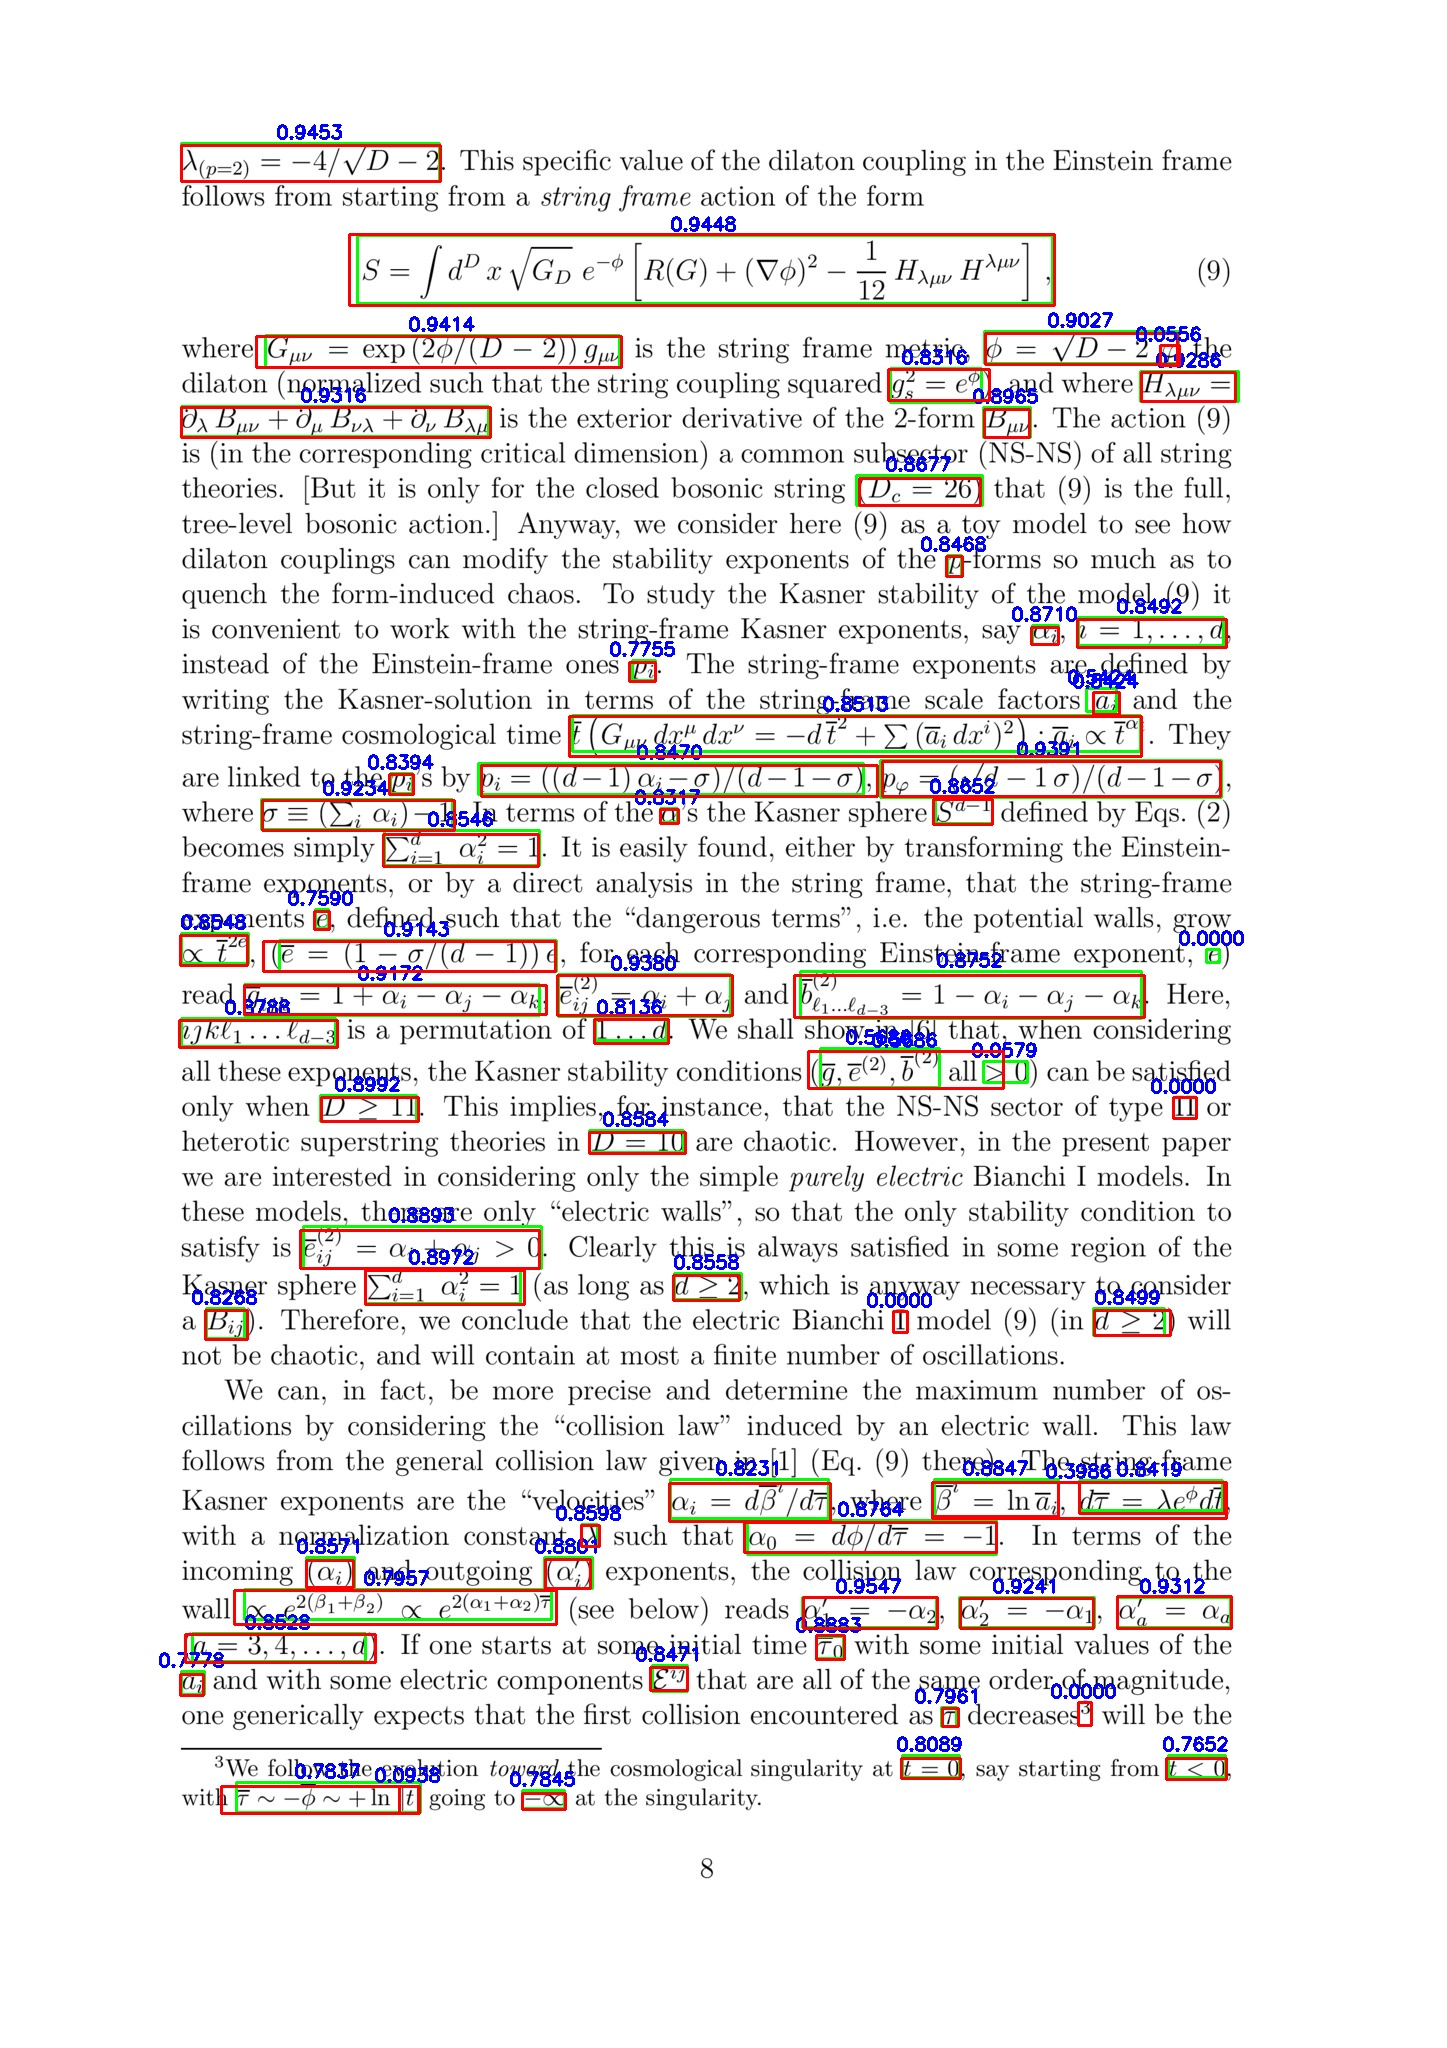
\includegraphics[scale=0.2]{intro/intro.jpg}}
\caption{Detection of mathematical formulas in PDF documents}
\end{figure}


% related works

\section{Related Works}
For many years, the detection of mathematical formulas has been recognized as a difficult task \cite{Chan2000}. There are several existing methods for detecting mathematical expressions in PDF documents using formatting information, for example page layout, character labels, character locations, font sizes, etc.  However, there are many different tools for generating PDF documents, and there are a variant in their character quality. Lin el al. \cite{Lin2011} shows that mathematical formulas can be a composition of some object types. For instance, the square root sign in a PDF generated by \LaTeX consists of the text object representing a radical sign and a graphical object for the horizontal line, which results the fact that some symbols must be identified from multiple drawing elements \cite{Mali2020}. \\
(to be continued...)

% method
\section{Method}
We use the Faster R-CNN model with ResNet50 as the backbone for our model. This is an object detection model, which consists of $2$ modules. The first module of the Faster R-CNN model is a deep fully convolutional network that proposes regions. The second module is a detector that uses proposed regions from the first one \cite{f-rcnn}. This is a single, unified network for object detection. By using the recently popular terminology of neural networks as the 'attention' mechanisms, the Region Proposal Networks (RPN) tells the Fast R-CNN where to look.

\begin{figure}[H]
\centering{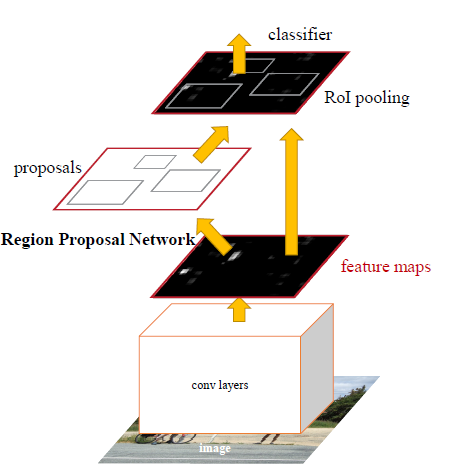
\includegraphics[scale=0.7]{faster-rcnn/faster-rcnn}}
\caption{Faster R-CNN is a single, unified network for object detection. The RPN module plays the role of the 'attention' of this network.}
\end{figure}

\subsection{Region Proposal Networks}
An RPN takes an image as input and outputs a set of rectangular object proposals each with an objectness score, which measures membership to a set of object classes. This process is modeled with a fully convolutional network. The structure of the RPN and an example are shown in Figure \ref{rpn}.

\begin{figure}[H]
\centering{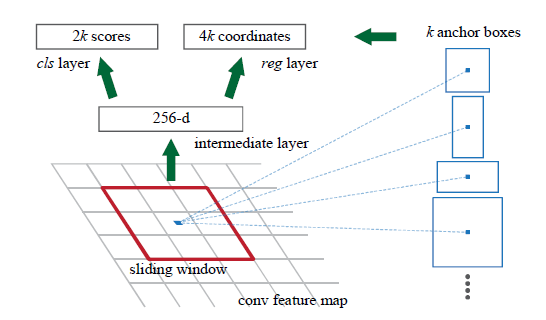
\includegraphics[scale=.8]{faster-rcnn/rpn}}
\caption{\textbf{Left:} RPN. \textbf{Right:} An example of detection using RPN.}
\label{rpn}
\end{figure}

\textbf{Loss function:} From \cite{f-rcnn}, the loss function of the RPN is:
$$L\left( {\left\{ {{p_i}} \right\},\left\{ {{t_i}} \right\}} \right) = \frac{1}{{{N_{cls}}}}\sum\limits_i {{L_{cls}}\left( {{p_i},p_i^*} \right) + \lambda \frac{1}{{{N_{reg}}}}\sum\limits_i {p_i^*} } {L_{reg}}\left( {{t_i},t_i^*} \right).$$

\subsection{Sharing Features for RPN and Fast R-CNN}
In the Faster R-CNN model, they use a 4-step training algorithm to learn shared features via alternating optimization. In the first step, the RPN is trained end-to-end by back-propagation and stochastic gradient descent (SGD). In the second step, they train a separate detection network by Fast R-CNN. In the third step, they use the detector network to initialize RPN training, and they let the two networks share convolutional layers. Finally, they keep the shared convolutional layers fixed, they fine-tune the unique layers of Fast R-CNN.


% experiments
In this section, we will describe the implementation of our mathematical formula detection system and dataset in detail.
\subsection{Dataset}
Our data is from the \href{https://zenodo.org/record/4757865}{IBEM dataset}. This originally comprises $600$ documents, with $8273$ pages in total. Those documents are parsed from mathematical papers, then each page is annotated with a bounding box of 2 types: isolated and embedded. The dataset is then split into various sets for ICDAR 2021 Competition on Mathematical Formula Detection, including Training, Test, and Validation sets. \\
\textbf{Training}
\begin{itemize}
\item Tr00: $4082$ pages.
\item Tr01: $760$ pages.
\item Tr10: $329$ pages.
\end{itemize}
\textbf{Test}
\begin{itemize}
\item Ts00: $736$ pages.
\item Ts01: $380$ pages.
\item Ts10: $699$ pages.
\item Ts11: $329$ pages.
\end{itemize}
\textbf{Validation}
\begin{itemize}
\item Va00: $577$ pages.
\item Va01: $380$ pages.
\end{itemize}
Our experiment uses Tr01, Tr10, Ts01 for training, Va01 for validation, and Ts11 for testing with $2178$ pages in total ($ \sim 26.33\% $ of the original dataset), and an approximate ratio of $4.47:1.16:1.$ The reason for this small subset is for the purpose of evaluating the ability of the model on small subsets, and the performance it gives (F1-score) through time (minutes).
\subsection{Implementation Details}
Our baseline model is Faster R-CNN with ResNet50 as the backbone. We have trained on Kaggle with a 4-core CPU, 12GB RAM, and a NVIDIA Tesla P100 GPU \footnote{\url{https://www.kaggle.com/docs/notebooks}}. The images are resized to $1447 \times 2048$ with the same ratio. The size of the region crops from the image is $1200 \times 1120$ to fit the limitation of the machine. They are also flipped and padded for data augmentation. For the feature aggregation, we use FPN (2-6). The loss function for the classifier is Cross-Entropy Loss and for the bouding box is L1 Loss. Test images are resized to $1583 \times 2048$ due to the distribution of the test dataset, flip augmentation is also applied. For post-processing, Non-Maximum Suppression (NMS) with $0.5$ IoU threshold to remove redundant boxes. All models are trained based on the MMDetection toolbox and config given by \href{https://github.com/Yuxiang1995/ICDAR2021_MFD/blob/main/configs/_base_/models/faster_rcnn_r50_fpn.py}{Yuxiang Zhong}. The optimizer for this baseline is Stochastic Gradient Descent (SGD) with a learning rate of $0.02.$  
\subsection{Remarks}
We have tested on 3 configs: Faster R-CNN with schedule 1x ($12$ epochs), \href{https://github.com/hkzhang95/DynamicRCNN}{Dynamic R-CNN} with schedule 1x ($12$ epochs) to check if it is better than the faster one and Faster R-CNN with schedule 2x ($24$ epochs) to check if the model is underfitting with low epochs. 
\begin{figure}[H]
\centering{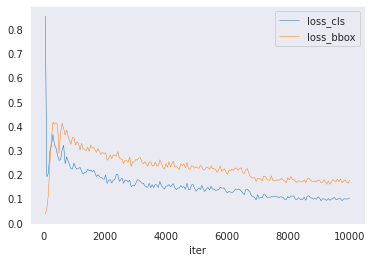
\includegraphics[scale=0.7]{loss/v2_1x}}
\caption{Faster R-CNN with schedule 1x}
\end{figure}

\begin{figure}[H]
\centering{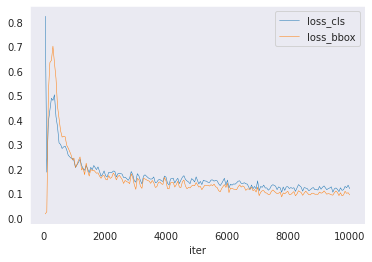
\includegraphics[scale=0.7]{loss/v5_1x}}
\caption{Dynamic R-CNN with schedule 1x}
\end{figure}

\begin{figure}[H]
\centering{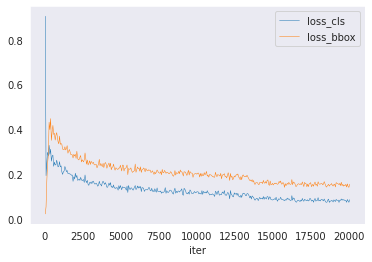
\includegraphics[scale=0.7]{loss/v2_2x}}
\caption{Faster R-CNN with schedule 2x}
\end{figure}

The F1-score gained from the model is as follow.
\begin{figure}[H]
\centering{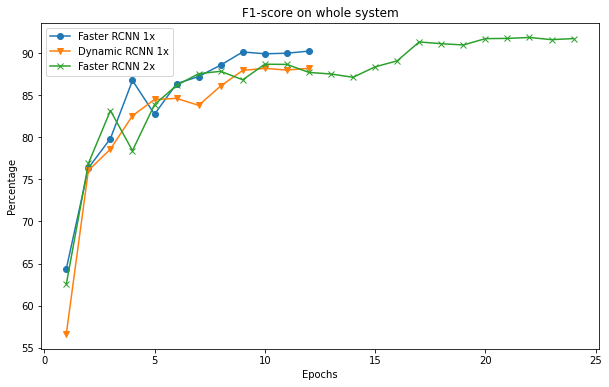
\includegraphics[scale=0.45]{f1-score/whole}}
\caption{F1-score on whole system}
\end{figure}

\begin{figure}[H]
\centering{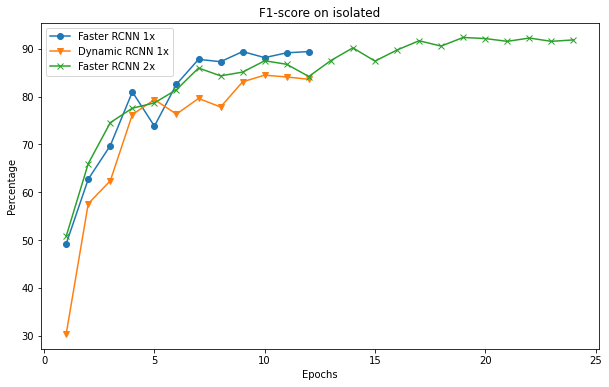
\includegraphics[scale=0.45]{f1-score/isolated}}
\caption{F1-score with isolated bounding box}
\end{figure}

\begin{figure}[H]
\centering{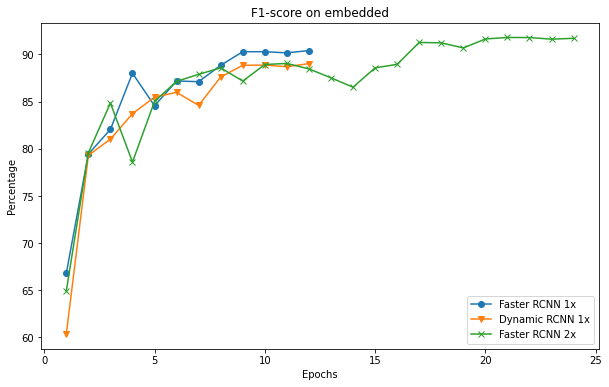
\includegraphics[scale=0.45]{f1-score/embedded}}
\caption{F1-score with embedded bounding box}
\end{figure}
It can be seen from the graphs that on the whole system, with the same schedule 1x, the F1-scores given by the Faster R-CNN model are higher than the one by Dynamic R-CNN if we use the same number of epochs, except in the case of $5$ epochs. The difference gets higher when we increase the number of epochs. Compared to the scores by Faster R-CNN with schedule 2x ($24$ epochs), although it gives a lower percentage when trained with a small number of epochs, the score becomes increasing to around $90\%$. 


% conclusion and future works
\section{Conclusion and Future Work}
%\section{Conclusion and Future Work}
In this paper, we presented our solution to the problem of mathematical formula detection in PDF documents. Our method was implemented with Faster R-CNN with ResNet50 as the backbone and improved by Feature Pyramid Network. We used about a quarter of the IBEM dataset for training, validation, and testing. Our model has significant results, with the highest F1-score being more than $90\%$ when tested with 3 configs on this dataset.

In the future, we intend to improve our model so that it can give better results when working with larger datasets. Moreover, based on this model, we want to build a model which can detect mathematical formulas in both PDF documents and image documents, as well as the model can transfer those formulas to \LaTeX commands, making it more convenient for people to re-type their scientific documents to \LaTeX.

% acknowledgements
\section*{Acknowledgment}
% \section*{Acknowledgment}
This paper and the research behind it would not have been finished unless there was brilliant support from our mentor, Mr. Dang Nguyen Hai. His enthusiasm, knowledge, and exacting attention to detail have been an inspiration and kept our work on track from our first approach to this topic to the final draft of this paper.

We show our gratitude to Assoc. Prof. Minh-Triet Tran and Assoc. Prof. Quan Vu Hai for sharing their pearls of wisdom with us during the course of this research, and we also thank them for their reviews of this paper.

We would also like to thank our classmates at the University of Science, Vietnam National University Ho Chi Minh City, who have looked over our manuscript and answered a variety of questions from us.

We are also immensely grateful to our friends for their comments on an earlier version of this transcription, although any errors are our own.

\nocite{*}

%\section*{References}
%\begin{thebibliography}{00}
% https://libraryguides.vu.edu.au/ieeereferencing/confernenceproceedings
%% \bibitem{b0} G. Eason, B. Noble, and I. N. Sneddon, ``On certain integrals of Lipschitz-Hankel type involving products of Bessel functions,'' Phil. Trans. Roy. Soc. London, vol. A247, pp. 529--551, April 1955.
% \bibitem{b-1} J. Clerk Maxwell, A Treatise on Electricity and Magnetism, 3rd ed., vol. 2. Oxford: Clarendon, 1892, pp.68--73.
\bibitem{b1} Zhong, Y., Qi, X., Li, S., Gu, D., Chen, Y., Ning, P., and Xiao, R. (2021). 1st Place Solution for ICDAR 2021 Competition on Mathematical Formula Detection.  Available: \url{http://arxiv.org/abs/2107.05534}.

%\end{thebibliography}
\printbibliography
\end{document}
